\documentclass[11pt,a4paper]{article}

\usepackage[margin=1in]{geometry}
\usepackage{times}
\usepackage{amsmath,amssymb}
\usepackage{graphicx}
\usepackage{booktabs}
\usepackage{hyperref}
\usepackage{natbib}
\usepackage{microtype}
\usepackage{xcolor}
\usepackage{caption}
\usepackage{subcaption}
\usepackage{float}
\usepackage{enumitem}
\usepackage{titlesec}
\usepackage{abstract}

\hypersetup{
  colorlinks=true,
  linkcolor=blue!60!black,
  citecolor=blue!60!black,
  urlcolor=blue!60!black
}

\titleformat{\section}{\large\bfseries}{\thesection.}{0.5em}{}
\titleformat{\subsection}{\normalsize\bfseries}{\thesubsection}{0.5em}{}
\titleformat{\subsubsection}{\normalsize\itshape}{\thesubsubsection}{0.5em}{}

\title{\textbf{Mechanistic Interpretability of Hybrid SSM-Attention Models:\\
Induction, Factual Recall, and Weight-Tied Attention in Zamba2-1.2B}}

\author{
  Mukund Pandey \\
  \textit{Independent Researcher} \\
  \texttt{mukund.pandey@gmail.com}
}

\date{}

\begin{document}

\maketitle

\begin{abstract}
State space models (SSMs) such as Mamba-2 are competitive with Transformers on language modeling benchmarks, yet their internal circuitry remains poorly understood. Hybrid architectures that interleave SSM layers with a small number of shared-weight attention blocks---such as Zamba2---compound this opacity: the same attention weights are reused at multiple depths, raising open questions about what each layer computes. We apply mechanistic interpretability methods to Zamba2-1.2B (38 layers: 32 Mamba-2 + 6 shared-attention hybrid), using hook-based residual stream analysis via TransformerLens. We introduce the \textbf{SSM Induction Score (SSMI)}, a logit-lens proxy for induction-like behavior in recurrent layers, and combine it with copy-score analysis and factual recall probing. Our main findings: (1) early hybrid layers (5, 11) implement induction heads (copy scores 0.669 and 0.485); (2) a middle hybrid layer (23) specializes in induction completion---producing the sharpest SSMI improvement (+8.9 log-prob units) despite near-zero copy score; (3) late hybrid layers (29, 35) specialize in factual recall, with peak accuracy at layer 35 (${\approx}96\%$ probability on correct token). Despite using identical QKV weights at all six positions, the shared attention block produces functionally distinct behavior at each depth, driven by the residual stream context it receives. This is, to our knowledge, the first mechanistic analysis of weight-tied attention in hybrid SSM architectures.
\end{abstract}

%%% ─────────────────────────────────────────────────────────────
\section{Introduction}

\subsection{The Interpretability Gap in Hybrid Models}

The mechanistic interpretability of Transformer language models has advanced considerably. We know that induction heads---attention heads that implement in-context copying via QK composition---emerge in early layers of GPT-2 and similar models \citep{olsson2022context}. We know that factual recall is mediated by mid-layer attention heads that move subject information to the final token position \citep{meng2022locating}. The interpretability toolkit---logit lens, activation patching, direct path decomposition---is mature for pure-attention architectures.

State space models do not have this foundation. Mamba-2 \citep{dao2024transformers} replaces attention with a structured state space recurrence, producing hidden representations that are not factored over input positions the way attention is. There is no attention matrix to inspect, no QK composition to analyze. The interpretability methods that work for Transformers require significant adaptation---or entirely new tools.

Hybrid architectures that interleave SSM layers with attention blocks are now production-grade. Zamba2 \citep{zyphra2024zamba2}, NemotronH \citep{nvidia2025nemotronh}, Jamba \citep{lieber2024jamba}, and Hymba \citep{nvidia2024hymba} all use this design. These models are widely deployed, yet essentially unanalyzed mechanistically. This paper addresses these questions for Zamba2-1.2B, the smallest publicly available hybrid model with a clearly documented architecture.

\subsection{The Shared-Weight Puzzle}

Zamba2's attention design is unusual: all six hybrid layers route through a \emph{single shared attention block} with identical QKV projection matrices. This raises a mechanistic question with no precedent in the Transformer literature: \textbf{can the same attention weights implement different computations at different depths?}

In standard Transformers, different layers specialize because they have different weights. In Zamba2, the weights are constrained to be identical. If specialization happens at all, it must emerge from the context---the residual stream---that the shared weights operate on, not from the weights themselves.

We show that specialization does happen, and characterize it precisely.

\subsection{Research Questions}

\begin{itemize}[leftmargin=1.5em]
  \item \textbf{RQ1:} Do Mamba-2 SSM layers develop induction-like behavior, and how does it build across layers?
  \item \textbf{RQ2:} Do the shared-weight attention blocks implement induction heads, and do all six implement the same circuit?
  \item \textbf{RQ3:} How do SSM and shared attention layers divide representational labor across task types?
\end{itemize}

\subsection{Contributions}

\begin{enumerate}[leftmargin=1.5em]
  \item \textbf{SSM Induction Score (SSMI):} A logit-lens proxy for induction-like behavior in recurrent layers. Requires one forward pass per sequence, practical on T4 hardware.
  \item \textbf{First copy-score analysis of weight-tied attention:} Copy scores for all 32 heads across all 6 hybrid layers in Zamba2-1.2B. Induction-head behavior concentrates in early hybrid layers (5, 11) and is absent later.
  \item \textbf{Functional specialization under weight tying:} Logit-lens probes on induction sequences and factual recall prompts show that the shared block implements different computations at layers 5/11, 23, and 35---driven entirely by residual stream context.
  \item \textbf{Open-source infrastructure:} TransformerLens adapters for Zamba2-1.2B (PRs \#1434, \#1486).
\end{enumerate}

%%% ─────────────────────────────────────────────────────────────
\section{Background}

\subsection{Mechanistic Interpretability in Transformers}

The residual stream serves as a shared scratchpad: each component reads from it and writes to it \citep{elhage2021mathematical}. This factored structure allows individual attention heads and MLP layers to be analyzed in isolation.

\textbf{Induction heads} \citep{olsson2022context} implement the algorithm: ``find the previous occurrence of the current token, then predict the token that followed it.'' The copy score---the mean attention weight from position $t$ to position $t - \text{prefix\_len}$---is the standard diagnostic; GPT-2 heads 4.4 and 5.5 have copy scores ${\approx}0.5$.

The \textbf{logit lens} \citep{nostalgebraist2020logitlens} applies the final layer norm and unembedding to intermediate residual stream states, revealing what each layer ``predicts'' if it were the final layer.

\subsection{State Space Models and Mamba-2}

Mamba \citep{gu2023mamba} replaces attention with a selective SSM: a recurrent computation where the state transition matrices are input-dependent. Mamba-2 \citep{dao2024transformers} restructures this via the structured state space duality (SSD), enabling efficient parallel training.

The key mechanistic consequence: there is no attention matrix to inspect, no QK composition to identify. If induction-like behavior exists in Mamba-2 layers, it must be mediated through hidden state compression and requires indirect detection methods.

\subsection{Hybrid Architectures}

Hybrid SSM-attention models inject attention at regular intervals to provide the key-value lookup capability that SSMs struggle with \citep{jelassi2024repeat}. \textbf{Zamba2-1.2B} \citep{zyphra2024zamba2} uses 38 layers: 32 Mamba-2 and 6 hybrid at positions $\{5, 11, 17, 23, 29, 35\}$, all sharing a single attention block (\texttt{num\_mem\_blocks=1}).

\subsection{TransformerBridge}

We contributed TransformerLens adapters wrapping Zamba2's HuggingFace model in the standard hook API (PRs \#1434, \#1486). The bridge exposes \texttt{run\_with\_cache} with \texttt{hook\_out} points at each residual block, enabling logit-lens and copy-score analyses with no model modifications. Layer type information must be read from \texttt{bridge.original\_model.config} (not \texttt{bridge.cfg}).

%%% ─────────────────────────────────────────────────────────────
\section{Methods}

\subsection{Models and Infrastructure}

We study \textbf{Zamba2-1.2B} \citep{zyphra2024zamba2}: 38 layers (32 Mamba-2, 6 hybrid at $\{5, 11, 17, 23, 29, 35\}$), shared attention with 32 heads, $d_\text{model}=2048$. All experiments run on a Google Colab T4 GPU (16GB) using TransformerBridge in \texttt{bfloat16}.

\subsection{SSM Induction Score via Logit Lens (SSMI)}

Standard induction detection uses attention patterns---not available for Mamba-2. We introduce SSMI: at each layer $L$, apply the final layer norm and unembedding to the cached residual stream output, then measure the log-probability assigned to the correct induction token.

\textbf{Test sequences:} ABC$\to$BCD sequences of the form \texttt{[prefix][SEP][prefix]}, where prefix is a random 30-token sequence. At each position $i$ in the second copy, the correct next token is \texttt{prefix[i - prefix\_len - 1]}. We use 10 sequences.

Formally:
\begin{equation}
  \text{SSMI}(L) = \frac{1}{|S| \cdot |P|} \sum_{s \in S} \sum_{i \in P_s} \log p_L(x_{i+1} \mid x_{0:i})
\end{equation}
where $p_L$ is the softmax distribution computed from layer $L$'s residual via logit lens. This requires only one \texttt{run\_with\_cache} call per sequence ($\approx$2 min for 10 sequences on T4).

\subsection{Shared Attention Copy Score}

For head $h$ in hybrid layer $l$, the copy score is:
\begin{equation}
  \text{CopyScore}(l, h) = \mathbb{E}_t\!\left[A_h[t,\; t - \text{prefix\_len} - 1]\right]
\end{equation}
where $A_h[t,s]$ is the attention weight from position $t$ to $s$, averaged over second-copy induction positions. We use 60 sequences with prefix length 40. Attention weights are extracted via \texttt{hf\_model(tokens, output\_attentions=True)}, which returns a 6-tensor tuple (one per hybrid layer).

\subsection{Factual Recall Logit Lens}

We apply the same logit-lens method to 13 factual recall prompts (capital cities, chemical symbols, historical facts), measuring per-layer log-probability of the correct single-token answer at the final prompt position.

%%% ─────────────────────────────────────────────────────────────
\section{Results}

\subsection{SSMI: Induction Signal Peaks at Layer 23}

\begin{figure}[H]
  \centering
  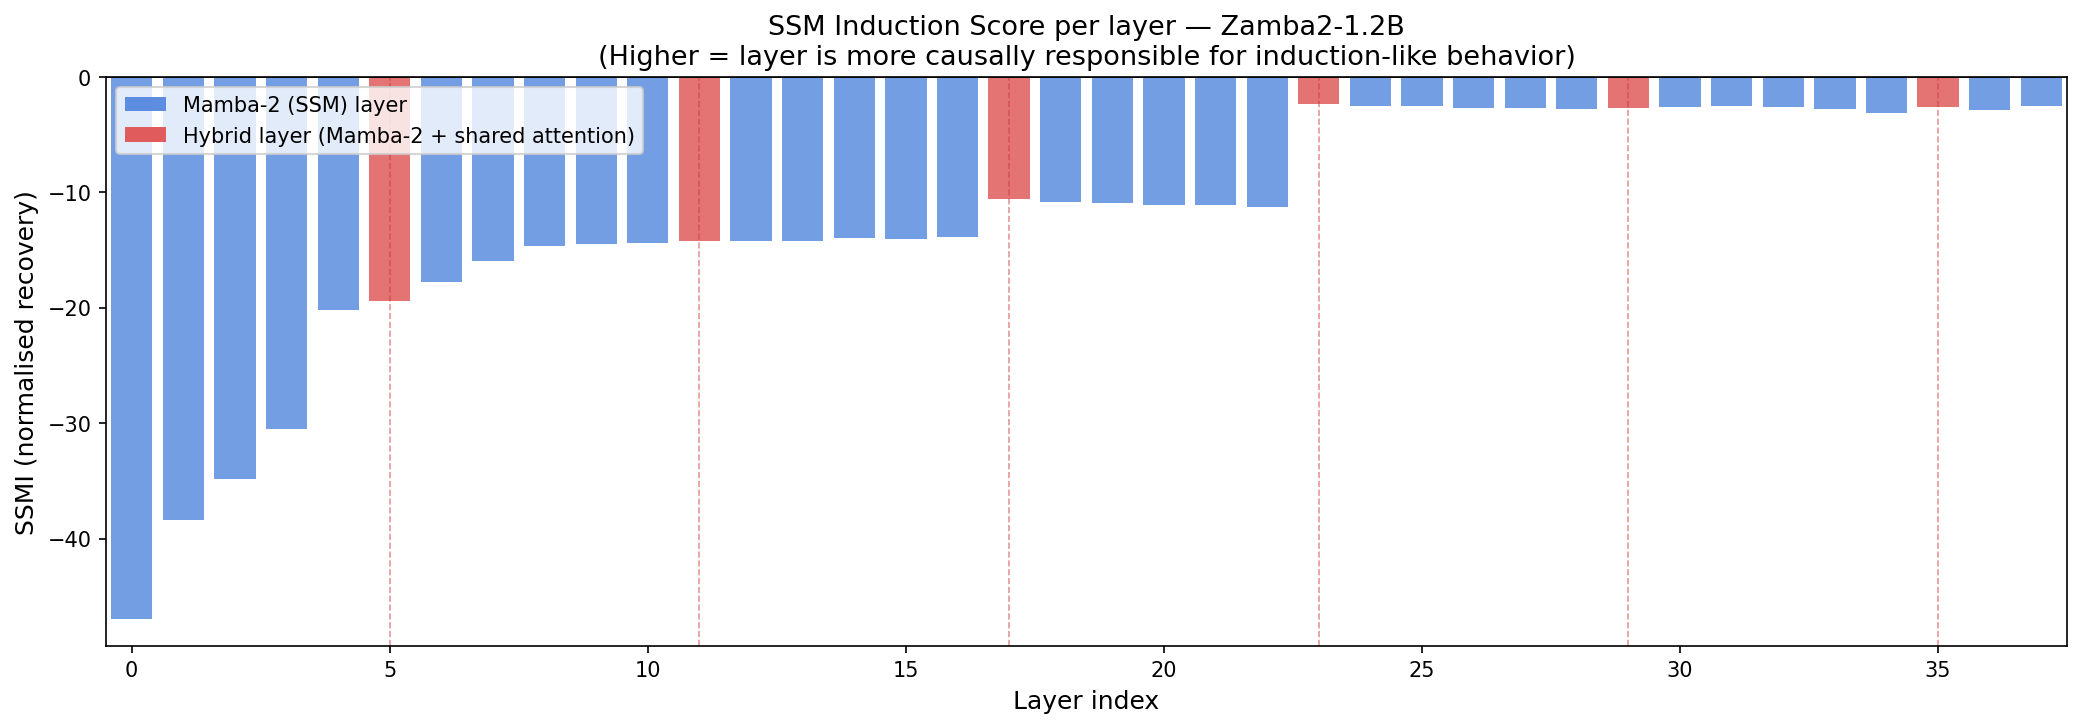
\includegraphics[width=\linewidth]{../figures/ssmi_zamba2_1.2b.png}
  \caption{SSM Induction Score (SSMI) per layer in Zamba2-1.2B. Red bars = hybrid layers; blue = Mamba-2. Vertical dashed lines mark hybrid layer positions. The sharp peak at layer 23 (+8.9 log-prob units improvement) is the dominant feature.}
  \label{fig:ssmi}
\end{figure}

SSMI rises monotonically from $-46.9$ (layer 0) to $-20.2$ (layer 4, just before the first hybrid layer). Each hybrid layer produces a discrete improvement. The largest single jump occurs at layer 23: SSMI rises from $-11.2$ to $\mathbf{-2.35}$---an improvement of 8.9 log-prob units, corresponding to ${\approx}9.5\%$ probability on the correct induction token vs. $3.4\%$ at layer 22.

\begin{table}[H]
  \centering
  \caption{SSMI summary statistics for Zamba2-1.2B.}
  \label{tab:ssmi}
  \begin{tabular}{lcc}
    \toprule
    Group & Mean SSMI & Best layer \\
    \midrule
    All Mamba-2 layers (32) & $-12.70$ & --- \\
    All Hybrid layers (6)   & $-8.64$  & --- \\
    Best single layer       & ---      & Layer 23 (hybrid), $-2.35$ \\
    \bottomrule
  \end{tabular}
\end{table}

\subsection{Copy Scores: Early Hybrid Layers Are Induction Heads}

\begin{figure}[H]
  \centering
  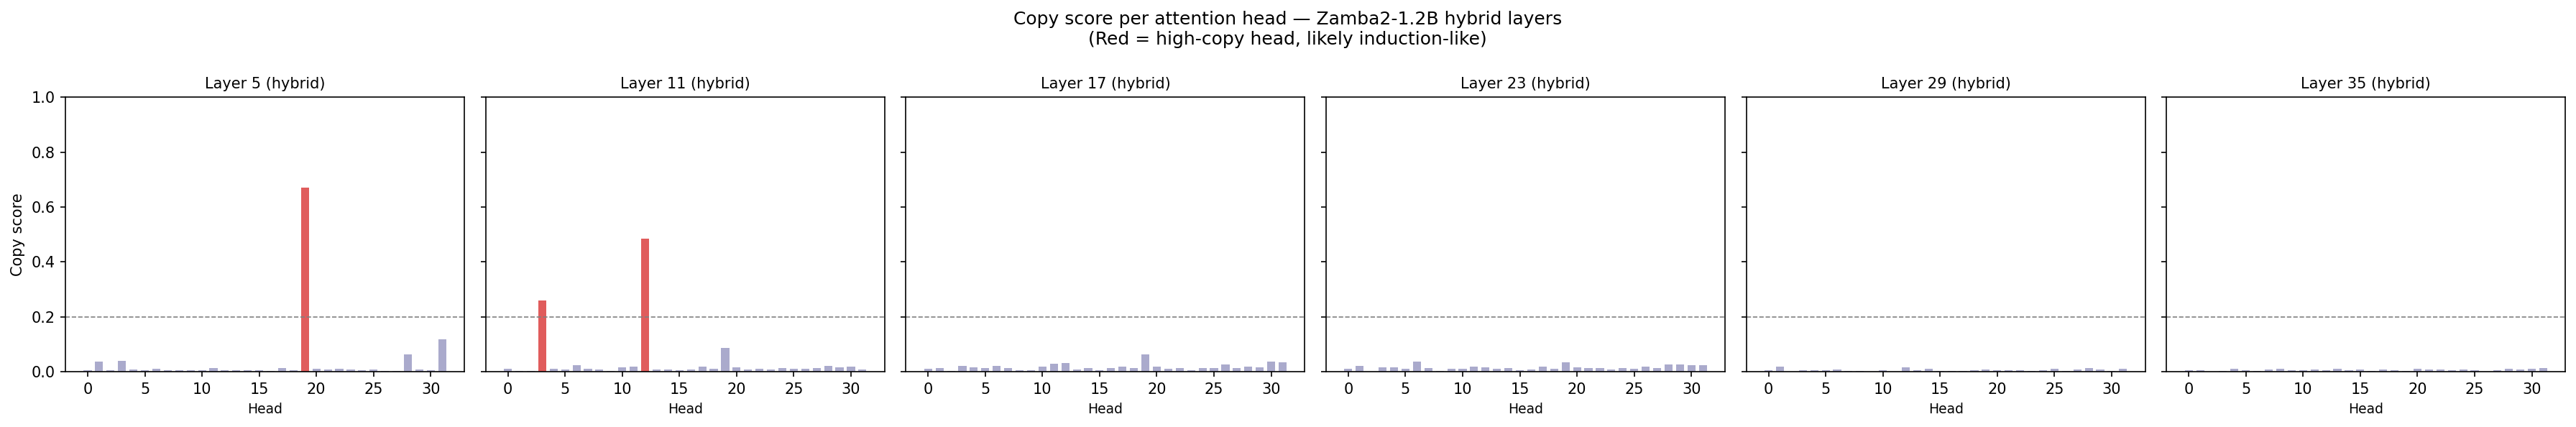
\includegraphics[width=\linewidth]{../figures/copy_scores_zamba2.png}
  \caption{Copy scores per attention head across all 6 hybrid layers. Induction-head behavior (score $>0.2$) is concentrated in layers 5 and 11; layers 17--35 show near-zero copy scores.}
  \label{fig:copy}
\end{figure}

\begin{table}[H]
  \centering
  \caption{High-copy heads (score $>0.2$) across hybrid layers. For comparison, GPT-2's strongest induction head (5.5) has copy score ${\approx}0.5$.}
  \label{tab:copy}
  \begin{tabular}{lccc}
    \toprule
    Layer & High-copy heads & Max score & GPT-2 comparison \\
    \midrule
    5  & Head 19           & 0.669 & Stronger than GPT-2 5.5 \\
    11 & Heads 3, 12       & 0.485 & Comparable to GPT-2 5.5 \\
    17 & ---               & 0.063 & --- \\
    23 & ---               & 0.037 & --- \\
    29 & ---               & 0.017 & --- \\
    35 & ---               & 0.013 & --- \\
    \bottomrule
  \end{tabular}
\end{table}

Despite identical QKV weights at all six positions, induction-head behavior concentrates entirely in layers 5 and 11. Layers 17--35 show near-zero copy scores. This demonstrates that the residual stream context at layers 5 and 11 is specifically suited to producing induction-like attention patterns from these weights.

\subsection{Factual Recall: Layer 35 Peaks, Not Layer 23}

\begin{figure}[H]
  \centering
  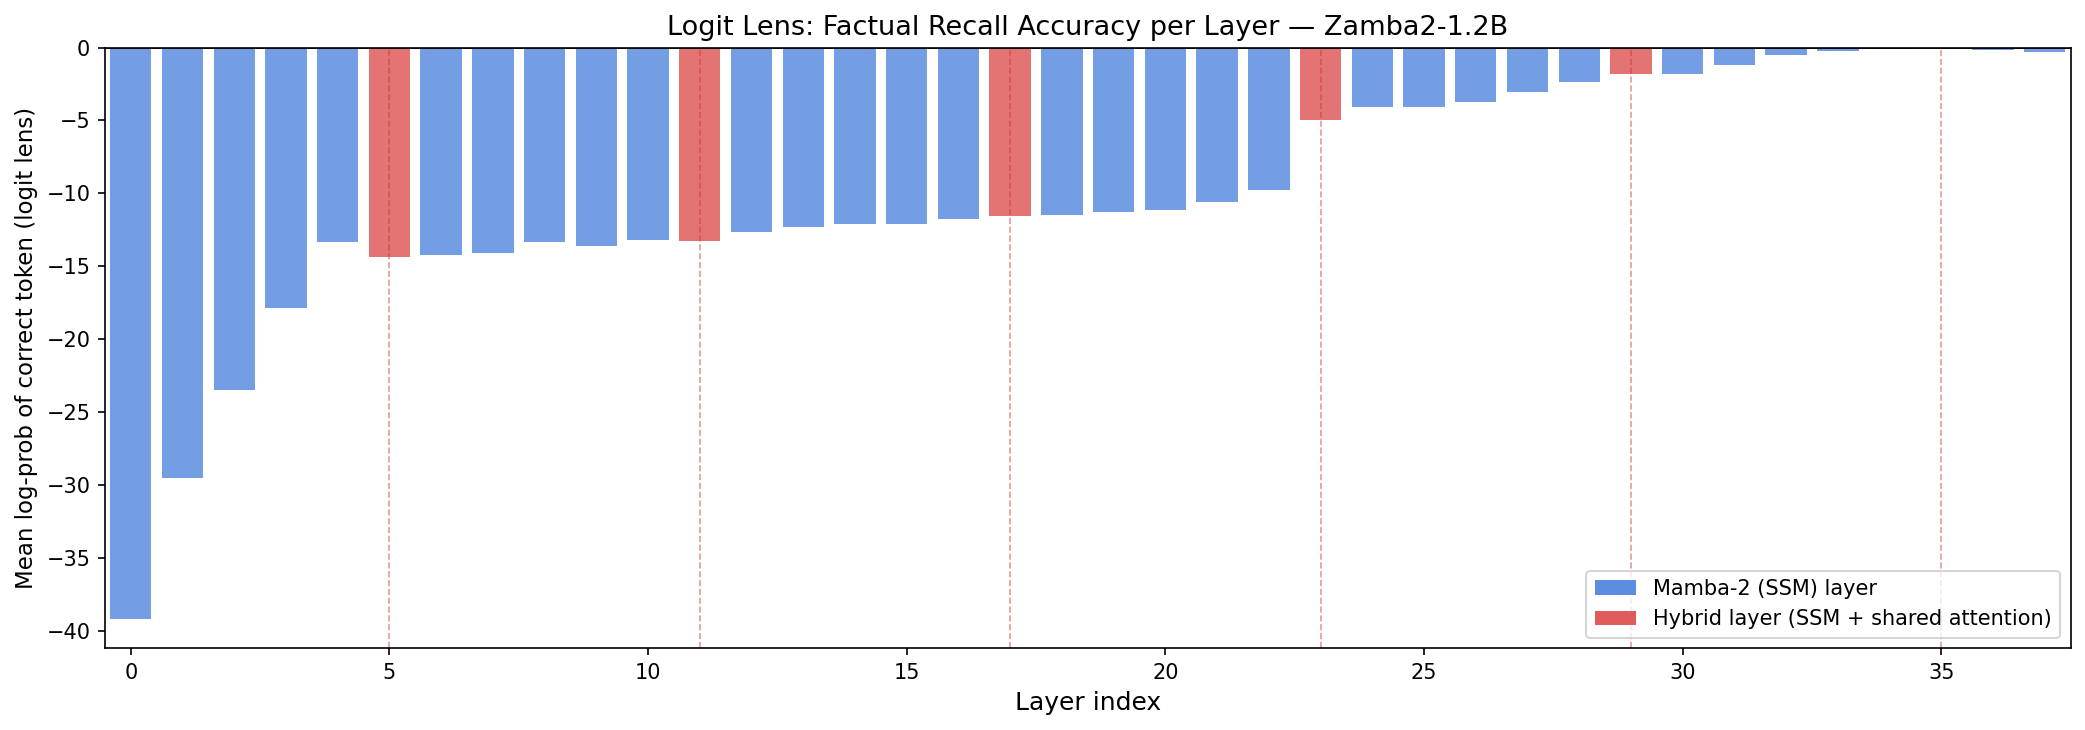
\includegraphics[width=\linewidth]{../figures/logit_lens_factual_zamba2.png}
  \caption{Logit-lens factual recall per layer. Unlike induction (Figure~\ref{fig:ssmi}), factual recall continues improving through all hybrid layers, peaking at layer 35 ($-0.043$ log-prob, ${\approx}96\%$ accuracy).}
  \label{fig:factual}
\end{figure}

\begin{table}[H]
  \centering
  \caption{Per-hybrid-layer comparison: SSMI (induction) vs. factual recall log-probabilities.}
  \label{tab:comparison}
  \begin{tabular}{lccc}
    \toprule
    Layer & Type & Factual recall logp & SSMI (induction) logp \\
    \midrule
    5  & hybrid & $-14.334$ & ${\approx}-19.4$ \\
    11 & hybrid & $-13.237$ & ${\approx}-14.2$ \\
    17 & hybrid & $-11.540$ & ${\approx}-10.6$ \\
    23 & hybrid & $-4.994$  & $\mathbf{-2.35}$ (peak) \\
    29 & hybrid & $-1.845$  & ${\approx}-2.8$ \\
    35 & hybrid & $\mathbf{-0.043}$ (peak) & ${\approx}-3.0$ \\
    \bottomrule
  \end{tabular}
\end{table}

Layer 23's large SSMI jump is \emph{specific to induction}---it does not appear in factual recall, where layer 23 shows only moderate improvement ($-4.994$). Factual recall keeps improving through layers 29 and 35, reaching near-certainty (${\approx}96\%$) only at the final hybrid layer.

\subsection{Revised Narrative: Seed $\to$ Amplify $\to$ Specialize}

The three experiments together support a coherent picture of how Zamba2-1.2B processes induction and factual recall:

\begin{enumerate}[leftmargin=1.5em]
  \item \textbf{Layers 0--4 (Mamba):} Basic sequence structure accumulated; SSMI rises from $-46.9$ to $-20.2$.
  \item \textbf{Layer 5 (hybrid):} Induction seeded via head 19 (copy score 0.669). Both tasks still poor.
  \item \textbf{Layers 6--10 (Mamba):} Signal amplified by SSM layers.
  \item \textbf{Layer 11 (hybrid):} Induction reinforced (heads 3, 12; copy scores 0.259, 0.485).
  \item \textbf{Layers 12--22 (Mamba):} Continued amplification; SSMI reaches $-11.2$.
  \item \textbf{Layer 23 (hybrid):} \textbf{Induction specialization.} Sharp SSMI jump ($+8.9$ logp); moderate factual recall gain.
  \item \textbf{Layer 29 (hybrid):} Factual recall continues improving ($-1.845$). Induction stable.
  \item \textbf{Layer 35 (hybrid):} \textbf{Factual recall resolution.} Peak at $-0.043$ (${\approx}96\%$).
\end{enumerate}

%%% ─────────────────────────────────────────────────────────────
\section{Discussion}

\subsection{Functional Specialization Under Weight Tying}

The core finding is that weight-tying does not prevent functional specialization. The same QKV weights implement copy heads at layers 5/11, induction consolidation at layer 23, and factual recall resolution at layer 35. The mechanism is straightforward: at each depth, the residual stream encodes qualitatively different information. QKV projections applied to position-heavy early residuals produce position-relative attention (induction heads). The same projections applied to semantically rich late residuals produce semantically structured attention (factual retrieval).

\subsection{Layer 23: Read Head, Not Copy Head}

Layer 23 shows the largest single-layer SSMI improvement ($+8.9$ logp) despite a copy score near zero. Our interpretation: by layer 23, the residual stream already encodes strong induction signal (built by Mamba layers 12--22 amplifying the layer 5/11 seeds). The shared attention at layer 23 does not need to implement copying; instead, it \emph{reads out} the induction signal already encoded, writing a sharp prediction into the residual stream. This is a ``read head'' rather than a ``write head.'' Testing this requires activation patching on the Q/K inputs to layer 23---left for future work.

\subsection{Limitations}

\textbf{Model scale:} Zamba2-1.2B is small; the layer-23/35 specialization may shift in larger variants.
\textbf{Factual recall sample:} 13 prompts is sufficient to identify the trend but not for quantitative variance claims.
\textbf{Logit lens approximation:} In models with residual stream drift, logit lens can distort early-layer estimates; relative comparisons are reliable, absolute scores less so.

%%% ─────────────────────────────────────────────────────────────
\section{Related Work}

\citet{olsson2022context} established induction heads as a core circuit in Transformer in-context learning. \citet{meng2022locating} located factual recall in mid-layer MLP weights via causal tracing. \citet{goldowsky2023localizing} introduced direct path patching for circuit-level analysis. Our work extends these methods to hybrid SSM architectures for the first time.

On SSM interpretability, \citet{ali2024hidden} analyze linear attention variants. We are not aware of prior work applying logit-lens or copy-score methods to Mamba-2 or hybrid models.

%%% ─────────────────────────────────────────────────────────────
\section{Conclusion}

We presented the first mechanistic interpretability analysis of a hybrid Mamba-2/shared-attention model. Using SSMI, copy-score analysis, and factual recall probing on Zamba2-1.2B, we identified three distinct functional roles for its six shared-attention hybrid layers:
(1) early layers (5, 11) seed induction via copy heads;
(2) layer 23 specializes in induction consolidation;
(3) layer 35 resolves factual recall.

The key insight is that \textbf{weight-tying does not prevent functional specialization}---the same QKV weights produce qualitatively different behavior at each depth because the residual stream context differs. This has implications for hybrid model design: weight-tied attention is not a ``tax'' on expressivity, but a mechanism that adapts to the computation already accumulated in the residual stream.

%%% ─────────────────────────────────────────────────────────────
\bibliographystyle{abbrvnat}
\bibliography{references}

\appendix

\section{Compute and Reproducibility}

All Zamba2-1.2B experiments were run on Google Colab T4 GPU (free tier). Total compute: ${\approx}3$ GPU-hours across three experiments. Code and notebooks are available at \url{https://github.com/mukundpandey/mech-interp-hybrid-ssm}.

\section{TransformerBridge Implementation Notes}

The \texttt{layers\_block\_type} field (list of \texttt{"mamba"} or \texttt{"hybrid"} per layer) must be read from \texttt{hf\_model.config}, not \texttt{bridge.cfg}. The bridge's \texttt{cfg} object is a TransformerLens \texttt{HookedTransformerConfig} and does not carry Zamba2-specific fields. All hook point names follow the pattern \texttt{blocks.N.hook\_out} for the residual stream output at layer $N$.

\end{document}
